%
% ---- contains strange adjustments search "goja"
%

%----------------------------------------------------------------------------------------
%	PACKAGES AND OTHER DOCUMENT CONFIGURATIONS
%----------------------------------------------------------------------------------------

\documentclass[
11pt, % Main document font size
a4paper, % Paper type, use 'letterpaper' for US Letter paper
oneside, % One page layout (no page indentation)
%twoside, % Two page layout (page indentation for binding and different headers)
headinclude,footinclude, % Extra spacing for the header and footer
BCOR5mm, % Binding correction
]{scrartcl}
%%%%%%%%%%%%%%%%%%%%%%%%%%%%%%%%%%%%%%%%%
% Arsclassica Article
% Structure Specification File
%
% This file has been downloaded from:
% http://www.LaTeXTemplates.com
%
% Original author:
% Lorenzo Pantieri (http://www.lorenzopantieri.net) with extensive modifications by:
% Vel (vel@latextemplates.com)
%
% License:
% CC BY-NC-SA 3.0 (http://creativecommons.org/licenses/by-nc-sa/3.0/)
%
%%%%%%%%%%%%%%%%%%%%%%%%%%%%%%%%%%%%%%%%%

%----------------------------------------------------------------------------------------
%	REQUIRED PACKAGES
%----------------------------------------------------------------------------------------

%\usepackage[
%nochapters, % Turn off chapters since this is an article        
%beramono, % Use the Bera Mono font for monospaced text (\texttt)
%eulermath,% Use the Euler font for mathematics
%pdfspacing, % Makes use of pdftex’ letter spacing capabilities via the microtype package
%dottedtoc % Dotted lines leading to the page numbers in the table of contents
%]{classicthesis} % The layout is based on the Classic Thesis style

%\usepackage{arsclassica} % Modifies the Classic Thesis package

\usepackage[T1]{fontenc} % Use 8-bit encoding that has 256 glyphs

\usepackage[utf8]{inputenc} % Required for including letters with accents

\usepackage{graphicx} % Required for including images
\graphicspath{{Figures/}} % Set the default folder for images

\usepackage{enumitem} % Required for manipulating the whitespace between and within lists

\usepackage{lipsum} % Used for inserting dummy 'Lorem ipsum' text into the template

%\usepackage{subfig} % Required for creating figures with multiple parts (subfigures)

\usepackage{amsmath,amssymb,amsthm} % For including math equations, theorems, symbols, etc

\usepackage{varioref} % More descriptive referencing

\usepackage{wrapfig}

\usepackage{caption}

\usepackage{subcaption}

%\usepackage[margin=0.5in]{geometry}

%----------------------------------------------------------------------------------------
%	THEOREM STYLES
%---------------------------------------------------------------------------------------

\theoremstyle{definition} % Define theorem styles here based on the definition style (used for definitions and examples)
\newtheorem{definition}{Definition}

\theoremstyle{plain} % Define theorem styles here based on the plain style (used for theorems, lemmas, propositions)
\newtheorem{theorem}{Theorem}

\theoremstyle{remark} % Define theorem styles here based on the remark style (used for remarks and notes)

%----------------------------------------------------------------------------------------
%	HYPERLINKS
%---------------------------------------------------------------------------------------

%\hypersetup{
%%draft, % Uncomment to remove all links (useful for printing in black and white)
%colorlinks=true, breaklinks=true, bookmarks=true,bookmarksnumbered,
%urlcolor=webbrown, linkcolor=RoyalBlue, citecolor=webgreen, % Link colors
%pdftitle={}, % PDF title
%pdfauthor={\textcopyright}, % PDF Author
%pdfsubject={}, % PDF Subject
%pdfkeywords={}, % PDF Keywords
%pdfcreator={pdfLaTeX}, % PDF Creator
%pdfproducer={LaTeX with hyperref and ClassicThesis} % PDF producer
%}

 % Include the structure.tex file which specified the document structure and layout

%Proposition using definition counter
\newenvironment{proposition}[1][]{\refstepcounter{definition}\par\medskip
   \noindent \textbf{Proposition~\thedefinition. #1} \rmfamily}{\medskip}
 

\begin{document}

%----------------------------------------------------------------------------------------
%	TITLE AND AUTHOR(S)
%----------------------------------------------------------------------------------------
\begin{titlepage}
\begin{center}
\begin{huge}
\vspace{1 in}
{\bf  Communication Efficient Data Exchange Among Multiple Nodes}\\  
\end{huge}
\vspace{0.5 in}
\begin{large}
\textbf{Midterm Report}\\
\textit{EP 299: Project \\for\\
M.Tech, Communication and Networks\\}
\end{large}
\begin{large}
\vspace{0.5cm}
{by\\}
\vspace{0.1cm}
{\bf Soumya Subhra Banerjee\\}
\end{large}
SR No. 04-02-04-37-42-16-1-14191\\
\vspace{.5in}

\begin{large}
{ Under the guidance of}\\
\end{large}
\vspace{0.2cm}
\begin{large}
{\bf Himanshu Tyagi,\\Assistant Professor}\end{large}
\vspace{1.0cm}

\begin{figure}[h]
\begin{center}


\includegraphics[width=4cm,height=4cm]{iisclogo}
%\caption{Result for the day}
%\label{fig:151106b_measure}
\end{center}
\end{figure}

\begin{large}
{ Department of Electrical Communication Engineering\\
Indian Institute of Science\\Bangalore - 560 012}\\
January 2018
\end{large}

\end{center}
\end{titlepage}

%----------------------------------------------------------------------------------------
%	TABLE OF CONTENTS & LISTS OF FIGURES AND TABLES
%----------------------------------------------------------------------------------------
\newpage
%\maketitle % Print the title/author/date block


\setcounter{tocdepth}{2} % Set the depth of the table of contents to show sections and subsections only

\tableofcontents % Print the table of contents
\newpage
\listoffigures

%----------------------------------------------------------------------------------------
%	ABSTRACT
%----------------------------------------------------------------------------------------
\newpage
\section*{Abstract}
Multiple parties observing correlated data seek to exchange their data using minimum communication. A practical method to achieve this has been proposed. \\In case the underlying joint distribution is known to the encoder a rate optimal solution to this problem is offered by Slepian-Wolf compression. In absence of this knowledge iterative and interactive communication is necessary to attain universal optimality. In both the cases joint decoding using type classes is of exponential complexity. However, Slepian-Wolf compression can be implemented using structured channel codes. We have considered implementation of the iterative Slepian-Wolf compression for two parties using Rateless Polar Codes where data exchange happens incrementally till completion. \\In this setting, interaction based on retransmission criterion offered by higher layers is not feasible.
Hence, we have  proposed a PHY-layer error detection scheme based on soft outputs of the Successive Cancellation decoder. We have presented simulation results that exhibit the performance of the considered methods.
Besides offering a solution to our problem, this scheme provides a CRC-free Rateless Polar Code which promises rate gain for short packet length communication.\footnote{This project is supported by Robert Bosch Center for Cyber Physical Systems}
 
%----------------------------------------------------------------------------------------
%	INTRODUCTION
%----------------------------------------------------------------------------------------
\newpage
\section{Introduction}\label{intro}
%----------Paper intro
Random correlated data (X,Y) is distributed between two parties with first observing X and second observing Y. The two parties seek to recover each others data. The \emph{Data-Exchange} problem essentially encompasses this scenario,  depicted in figure \ref{fig:dataex}. This project seeks to device a practical protocol which achieves this with minimal communication under a setting where the joint distribution of X and Y is unknown.\\
\begin{wrapfigure}{r}{0.5\textwidth}
  \begin{center}
    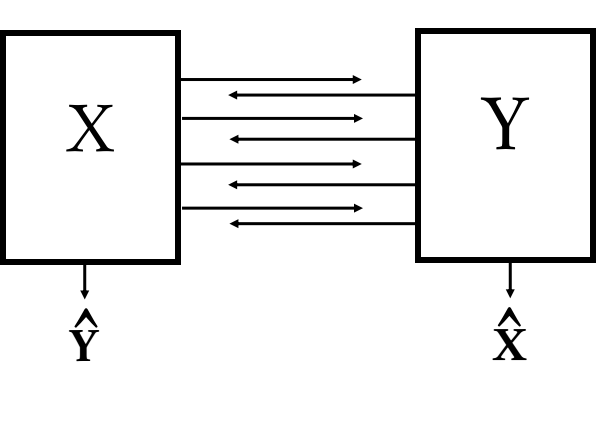
\includegraphics[width=0.4\textwidth]{dataex.png}
  \end{center}
  \caption{The Data-Exchange problem}
  \label{fig:dataex}
\end{wrapfigure}
A working solution to this problem is r-sync protocol, as described in   \cite{rsync}. The algorithm identifies parts of the source file which are identical to some part of the destination file, and only sends those parts which cannot be matched in this way. Though this protocol is fast and has low complexity, it does not exploit the correlation of the data to the best extent possible. In fact, we can view r-sync as an algorithm which uses only one guess,  thus ends up using more communication.\\
In \cite{sw}, David Slepian and Jack Wolf had shown that the optimal solution to this problem is Slepian-Wolf (SW) compression. 
\begin{wrapfigure}{r}{0.4\textwidth}
  \begin{center}
    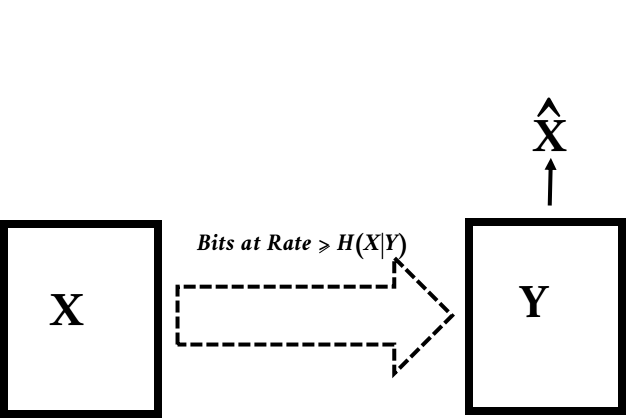
\includegraphics[width=0.4\textwidth]{swcomp.png}
  \end{center}
  \caption{The Slepian-Wolf compression}
  \label{fig:swcomp}
\end{wrapfigure}
\paragraph{Slepian-Wolf coding theorem:}It states that under joint decoding of X and Y a total rate H(X,Y) is sufficient for exchange of data.\\
As described in \cite{discus}, consider first the problem where X and Y are correlated discrete-alphabet memoryless sources, we have to compress X losslessly, with Y (side information) being known at the decoder and \emph{not} at the encoder. If Y were known at both ends one can compress X at a theoretical rate of $H(X|Y)$. But if Y were known only at decoder the same can be achieved by just knowing $P_{X|Y}$ at encoder without explicit information of Y, this has been depicted in figure \ref{fig:swcomp}. 
%goja
\clearpage
A practical implementation of Slepian-Wolf compression faces the following difficulties.
\begin{itemize}
\item Search is over an exponential list in decoding.
\item Knowledge of $P_{X|Y}$ is required at encoder.
\end{itemize} 

Using structured channel codes as indicated in \cite{discus}, particularly Polar Codes as shown in \cite{pslep}, along with \emph{recursive data exchange} protocol  mentioned in \cite{htsw} for SW compression eases the aforementioned implementation. 

\subsection{Suggested Approach for Solving The Data-Exchange Problem}\label{suggapp}
In accordance with the above discussion the suggested approach towards solving the \emph{Data-Exchange} problem may be briefed as follows.
\begin{itemize}
\item{Implement SW Compression using Polar Codes.}
\item{Achieve universality using \emph{recursive data exchange} protocol (RDE).}
\item{Realize RDE using Rateless Polar Codes with physical layer error detection.}
\end{itemize}

The following subsections discuss the artifacts needed for this implementation in brief. Section \ref{propsol}, consolidates and elaborates the proposed scheme. 

\subsection{Recursive Data Exchange Protocol}
The data exchange protocol is based on an interactive version of the SW protocol where the length of communication is increased in steps until the second party decodes the data of the first. After each transmission second party sends ACK-NACK feedback signal, the protocol stops when ACK is received or some fixed number of bits have been transmitted \cite{htsw}. Note, this protocol is universal as it does not rely on knowledge of the joint distribution, instead uses an iterative variable length approach to reach rate optimality universally. The decoders suggested in \cite{htsw} are theoretical constructs which use type classes to form a list of guesses for data of other parties and thus has exponential complexity.\\ In \cite{pslep}, SW compression is approached with Polar Codes, in this work we use Rateless Polar Codes to implement RDE with a similar ideology.
%goja
\clearpage
\subsection{Brief Introduction to Polar Codes}
\begin{wrapfigure}{r}{0.5\textwidth}
  \begin{center}
    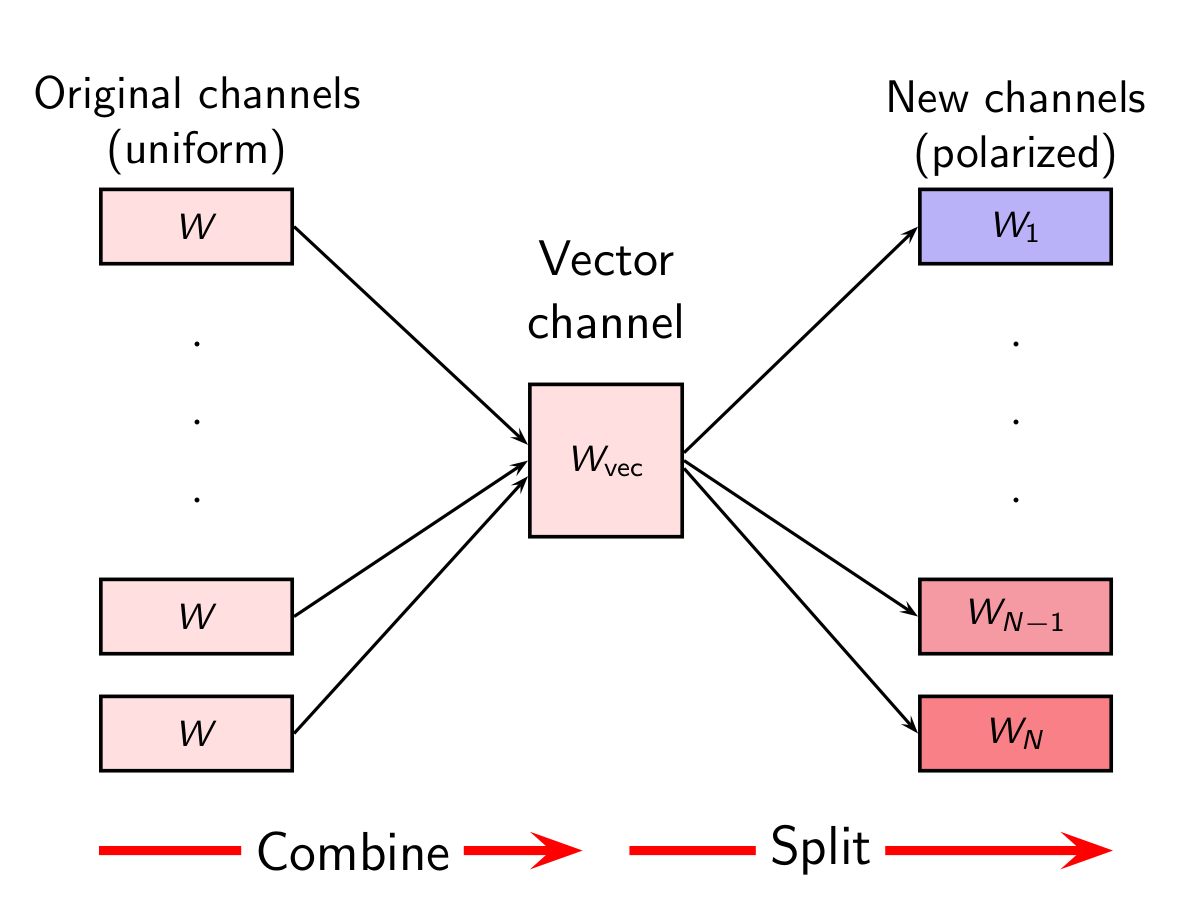
\includegraphics[width=0.4\textwidth]{channelcomb.png}
  \end{center}
  \caption{Channel combining and splitting}
  \label{fig:channelcomb}
\end{wrapfigure}
In 2008, E. Arikan in his paper \cite{arikan} introduced Polar Codes, which provably achieves capacity on symmetric channels. Polar Codes rely on the phenomenon of channel polarization which can be described as follows.
\begin{wrapfigure}{r}{0.5\textwidth}
  \begin{center}
    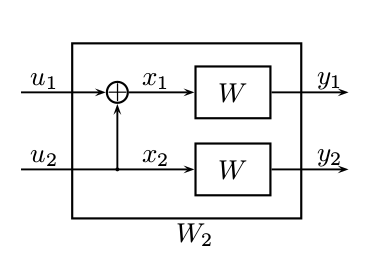
\includegraphics[width=0.4\textwidth]{arikanfly.png}
  \end{center}
  \caption{Arikan transformation butterfly}
  \label{fig:arikanfly}
\end{wrapfigure}
\paragraph{Channel Polarization:} It is an operation by which one manufactures out of $N$ independent copies of a given B-DMC ($W$), a second set of $N$ channels $\{W^{(i)}_N : 1 \leq i \leq N \}$ that show a polarization effect in the sense that, as $N$ becomes large, the symmetric capacity terms $I(W^{(i)}_N )$ tend towards $0$ or $1$, for all but a vanishing fraction of indices $i$. Hence, the Bhattacharya parameter $Z(W^{(i)}_N)$ tends to $1$ or $0$ respectively. The channels with $Z(W^{(i)}_N)=0$ captures the capacity of $W_{vec}$.

This operation consists of a channel combining and a channel splitting phase, as shown in figure \ref{fig:channelcomb}. The channel transformation for two independent channels is shown in \ref{fig:arikanfly}, which is used recursively. \\The encoding process sends data on transformed channels with $Z(W^{(i)}_N)=0$  (\emph{good channels}) and treats the channels with $Z(W^{(i)}_N)=1$ as \emph{frozen}, sending no useful data on them. This scheme of error control coding with Polar Codes is illustrated in figure \ref{fig:pchscheme}.
In figure \ref{fig:pchscheme}, $U_N$ is a uniform message vector, $T$ is a linear transform equivalent to the butterfly in figure \ref{fig:arikanfly} for a block length of $N$. $W_N$ is analogous to $W_{vec}$. It is useful to note here that $T=T^{-1}$.
\begin{figure}[h!]
 \begin{center}
    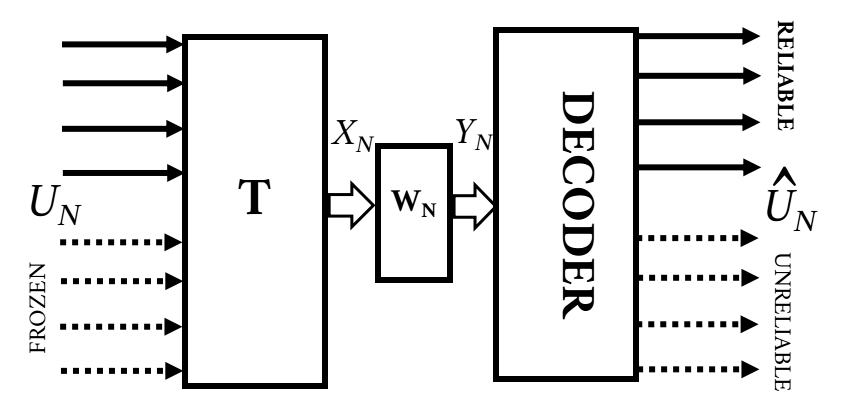
\includegraphics[width=0.6\textwidth]{pchscheme.png}
  \end{center}
  \caption{Polar Coding}
  \label{fig:pchscheme}
\end{figure}
In figure \ref{fig:pchscheme}, $U_N$ is a uniform message vector, $T$ is a linear transform equivalent to the butterfly in figure \ref{fig:arikanfly} for a block length of $N$. $W_N$ is analogous to $W_{vec}$. It is useful to note here that $T=T^{-1}$.
\begin{figure}[h!]
  \begin{center}
    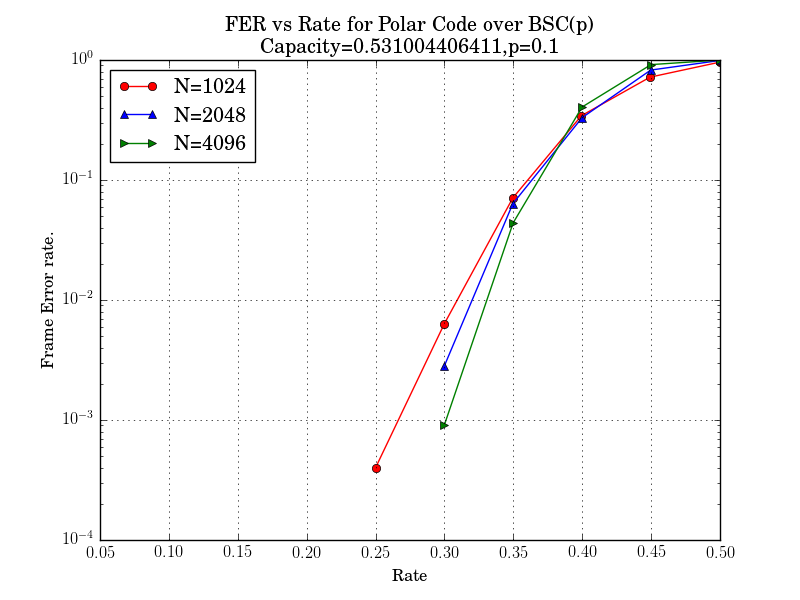
\includegraphics[width=0.6\textwidth]{fer.png}
  \end{center}
  \caption{FER vs Rate for Polar Coding with SC-decoding}
  \label{fig:fer}
\end{figure}
For our purpose, we shall be using Successive Cancellation (SC) decoding. Each independent channel will considered as BSC(p). The Polar Code construction indicated in \cite{zhang} has been employed for simplicity. A performance analysis of implementation of the scheme in figure \ref{fig:pchscheme} is presented in figure \ref{fig:fer}.   

\subsection{Implementation of SW Compression using Polar Codes}\label{psw}
In \cite{discus}, the use of structured codes for SW compression has been discussed. Further, in \cite{pslep} a specific scheme using Polar Codes has been illustrated, as shown in figure \ref{fig:pswscheme}.
\begin{figure}[h!]
 \begin{center}
    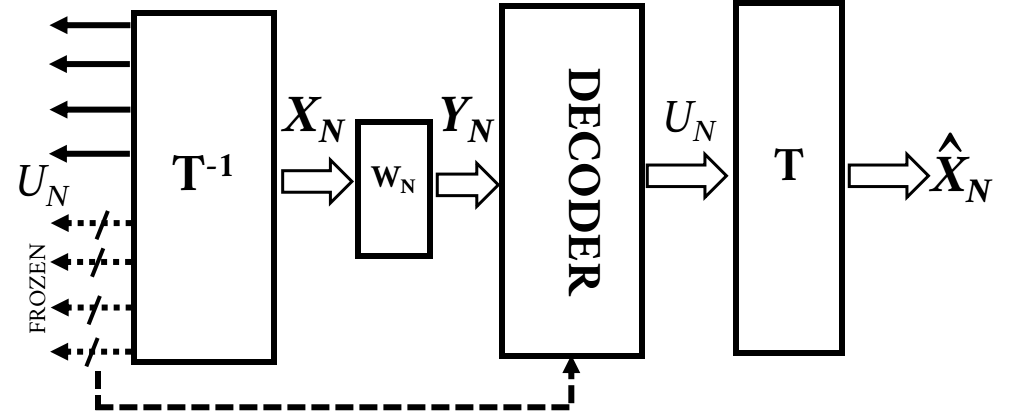
\includegraphics[width=0.6\textwidth]{pswscheme.png}
  \end{center}
  \caption{Polar Coding for SW compression}
  \label{fig:pswscheme}
\end{figure}\\
\begin{wrapfigure}{r}{0.5\textwidth}
 \begin{center}
    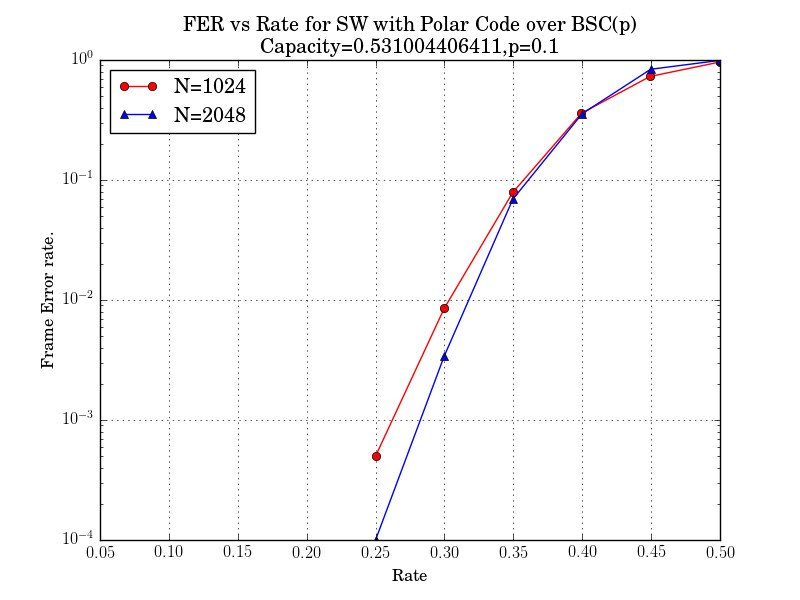
\includegraphics[width=0.6\textwidth]{swfer.png}
  \end{center}
  \caption{FER vs Rate for SW compression with Polar Code}
  \label{fig:swfer}
\end{wrapfigure}
Consider the setting where $X_N$ and $Y_N$ are uniform. $Y_N$ is a corrupted version of $X_N$ by $N$ BSC(p) channels. The bits that are to be sent for estimation of $X_N$ from $Y_N$ are the frozen bits in $U_N$. In other words applying $T^{-1}$ to $X_N$ and choosing the bits at frozen positions (the syndrome) essentially describes the compression operation. These bits are communicated error free to the SC-decoder. Thus $H(X_N)-I(W_N)=H(X_N/Y_N)$ bits are sent. On applying $T$ to the output of SC-decoder the estimate $\hat{X}_N$ is received. It is to be noted here that in general the frozen positions are set to $0$ in channel coding but in SW compression they are non-zero by the nature of the scheme. Performance analysis of this scheme is presented in figure \ref{fig:swfer}.

Intuitively, a method to generate the syndrome incrementally will lead us to an implementation of RDE. Rateless Polar Codes will be instrumental to accomplish this.
\clearpage
\subsection{Rateless Polar Codes}
\paragraph{Rateless Code:}A rateless coding scheme transmits incrementally more and more coded bits over an unknown channel until all the information bits are decoded reliably by the receiver. A fixed rate code is designed for a specific channel. In contrast, a rateless code is designed for a set of channels and judged for its performance for the entire set (the compound channel). In general a rateless code design is based on Hybrid-ARQ (HARQ) techniques and uses code puncturing. \\For Polar Codes, puncturing is not straightforward. HARQ schemes and puncturing of Polar Codes has been proposed and compared in \cite{harqtav}, \cite{harqcheng} and \cite{harqchen}.\\ In \cite{chen}, the authors have proposed a provably capacity achieving rateless coding scheme based on Polar Codes. This scheme is useful for broad class of channels as long as they are ordered by degradation\footnote{using construction methods in \cite{wang}, \cite{mondelli} this method can be extended to a broader class of \emph{less noisy} ordered channels}. The scheme stems from the inherent nesting property and degradedness of Polar Codes.

\subsubsection{Degradedness and Nesting Property}
\begin{wrapfigure}{r}{0.5\textwidth}
  \begin{center}
    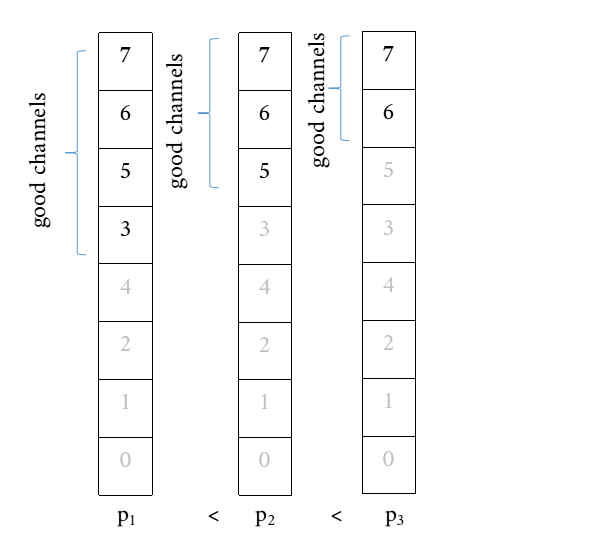
\includegraphics[width=0.5\textwidth]{relorder.png}
  \end{center}
  \caption{Nesting in BSC($p$) channels}
  \label{fig:relorder}
\end{wrapfigure}
\paragraph{Degraded Channels:}A symmetric binary input channel $W_2$ is said to be degraded with respect to a channel $W_1$ if there exists random variables X, Y, Z such that X\---Y\---Z forms a Markov chain and $W_1=P_{Y|X}$, $W_2=P_{Z|X}$. By data processing inequality it is evident that the capacity of $W_2$ is lesser than that of $W_1$. This is denoted by $W_2 \preceq W_1$. For example, $BSC(p_1) \preceq BSC(p_2)$ if $p_1 \geq p_2$.
\paragraph{Nesting Property:}Polarization suggests that $W_2 \preceq W_1$ will reflect as lesser number of \emph{good channels} for $W_2$. As the polarization operation preserves degradedness \cite{wang}, the good bit indices of $W_2$ must be a subset of the good bit indices of $W_1$. This is nesting property. 
%goja
\clearpage
This leads to a \emph{reliability ordering} of the bit-channels, such that a more reliable bit-channel is always noiseless if a less reliable bit-channel is noiseless regardless of the underlying channel.
\subsubsection{Incremental Freezing}\label{if}
Given the reliability ordering, the rateless scheme in \cite{chen} can be described as follows. The initial transmission can be done using a high rate Polar Code with many information bits and less frozen bits. If this transmission cannot be decoded\footnote{Decodability is checked by CRC in higher layers.} then among the informations bits sent, the ones on comparatively lesser reliable channels are retransmitted. By decoding these bits from future transmissions they effectively become frozen, allowing the rest of the information bits sent on the first transmission to be decoded.  As future transmissions successively freeze more and more bits sent in earlier transmission, this scheme can be called \emph{Incremental Freezing} (Inc-Frz).
\begin{figure}[h]
 \begin{center}
    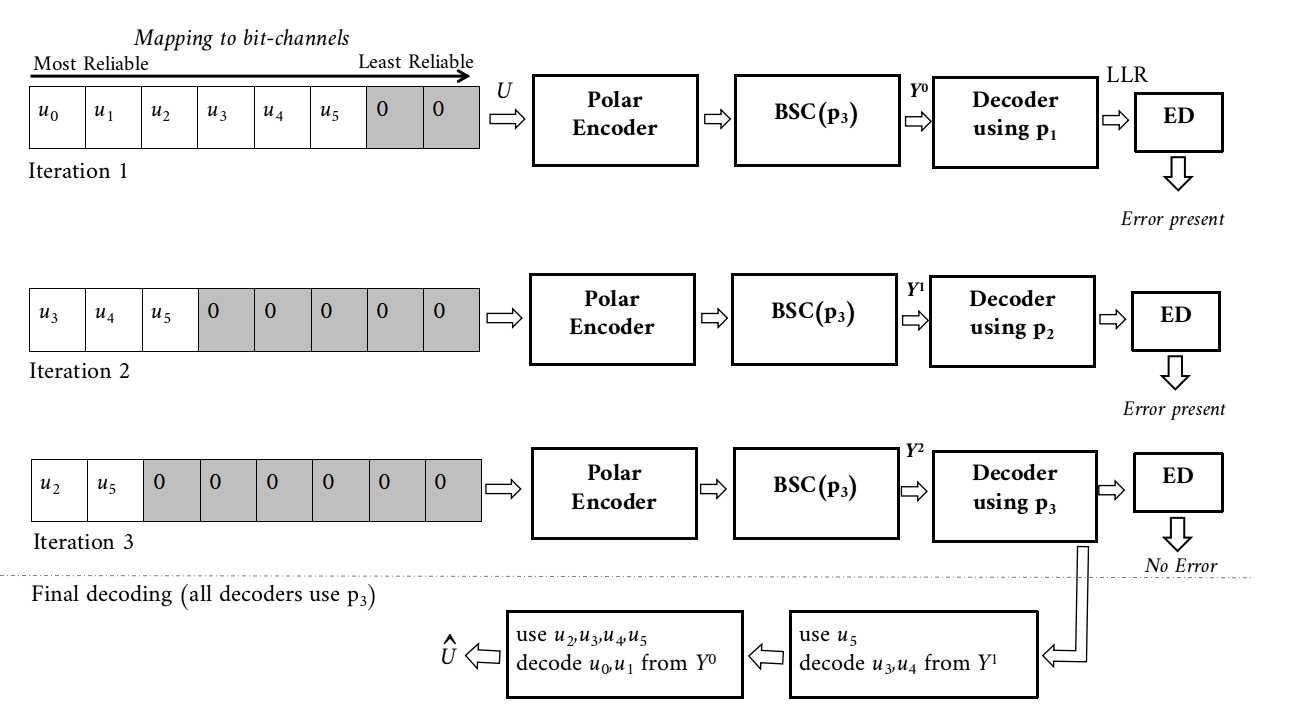
\includegraphics[width=1\textwidth]{if2.png}
  \end{center}
  \caption{Incremental Freezing for $N=8$, $K=6$ and $3$ iterations}
  \label{fig:if}
\end{figure}  
\\Figure \ref{fig:if} illustrates the scheme for a set of channels with rates $\{ R_1=6/8, R_2= R_1/2=3/8,R_3= R_1/3=1/4\}$. Here $u_i$ are the message bits. Note that with the $3^{rd}$ transmission  $u_2$ to $u_{5}$ have been incrementally frozen. This scheme is capacity achieving in the sense that no rate has been wasted, the final rate achieved is, $$R^*= \frac{6}{8*3}=\frac{1}{4}=R_3 $$ In case the real channel has capacity $ \geq R_3$ the scheme stops at appropriate iteration to achieve that capacity.\\
Though this scheme is not truly rateless as it can achieve only $R$, $R/2$, $R/3$,... rather than a set of arbitrary rates, adding new information bits in future transmissions allow us to rectify this. In similar fashion this can be extended to parallel channels.\\
It is useful to note that a certain number of channels in this scheme is "\emph{always available}" guaranteeing a certain rate in each transmission. An application of this will be discussed in section \ref{future}.
\\In \cite{chen}, The performance evaluation of the scheme establishes that $n$ iterations of the scheme is almost equivalent in performance to a $R/n$ fixed rate Polar Code.
\\Adaptation of this scheme for RDE will be indicated in section \ref{propsol}.
\\The following subsections briefly discuss Rateless Polar Coding from the perspective of HARQ.
\subsubsection{HARQ for Polar Codes}
\paragraph{Hybrid ARQ:}Hybrid automatic repeat request (hybrid ARQ or HARQ) is a combination of high-rate forward error-correcting coding and ARQ error-control. In standard ARQ, redundant bits are added to data to be transmitted using an error-detecting (ED) code such as a cyclic redundancy check (CRC). Receivers detecting a corrupted message will request a new message from the sender. \\In Hybrid ARQ, the original data is encoded with a forward error correction (FEC) code, and the parity bits are either immediately sent along with the message (Type-I) or only transmitted upon request when a receiver detects an erroneous message (Type-II). The retransmission vector is also known as the \emph{Redundancy Vector} (RV). \\The ED code may be omitted when a code is used that can perform both forward error correction (FEC) in addition to error detection, such as a Reed-Solomon code or  Turbo Product Code (TPC) \cite{harqmukhtar}.\\The FEC code is chosen to correct an expected subset of all errors that may occur, while the ARQ method is used as a fall-back to correct errors that are uncorrectable using only the redundancy sent in the initial transmission.\\Construction of HARQ requires a Rate Compatible Code and a choice of RV.
\paragraph{Rate Compatible Codes:}
Given a fixed number of information bits, consider a family of codes $\{C_1,C_2...C_n\}$  with rates $R_1\geq R_2\geq R_3...\geq R_n$, and block lengths $N_1 \leq N_2 \leq ... \leq N_n$.
Then the set is rate compatible if codeword for $C_i$ can be built by removing $N_j-N_i$ bits from codewords of code $C_j$ , $j\geq i$, \cite{mondelli}. Rate Compatible Codes can be constructed by puncturing low rate codes. 
\\Polar Codes for degraded channels are inherently rate compatible due to reliability ordering and nesting.

\subsubsection*{HARQ Schemes for Polar Codes}
\begin{wrapfigure}{r}{0.5\textwidth}
  \begin{center}
    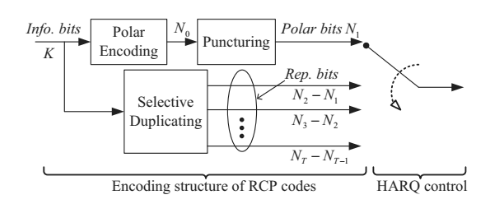
\includegraphics[width=0.5\textwidth]{selrepharq.png}
  \end{center}
  \caption{HARQ for Polar Codes with selective repetition}
  \label{fig:selrepharq}
\end{wrapfigure}
In \cite{harqchen}, a HARQ scheme for Polar codes based on selective repetition has been studied. The Incremental Freezing scheme described in \cite{chen} and \cite{mondelli} can be classified as a HARQ scheme. In \cite{harqtav} another H-ARQ scheme based on Subset Polar Codes is described along with performance comparison with the other schemes. Here these schemes are discussed in brief.            
\\\paragraph{Selective Repetition:}
As the initial transmission, an information block of $K$ bits is fed into a polar
encoder. The output codeword of $N_0$ bits is punctured into $N_1$
bits and sent over the channel. If the receiver fails to decode
the codeword, an NACK (negative acknowledgement) is sent
to the transmitter through the feedback channel. And then,
$N_2-N_1$ of the information bits are retransmitted. This time,
the receiver tries to perform decoding with all the $N_2$ received
bits. If the decoding is failed again, another $N_3-N_2$ bits
are transmitted. This process continues until the transmitter
receives an ACK (acknowledgement), or a maximum number
of transmissions $T$ is achieved. The scheme has been illustrated in figure  \ref{fig:selrepharq}. The retransmitted bits (RV) are chosen one at a time as the most unreliable of the $K$ bits transmitted, reliability is calculated after choosing one bit and the process is iterated.
\paragraph{Incremental Freezing:} This scheme is an improvement over the above scheme, it uses the reliability ordering to choose the RV as discussed in \ref{if}.
\paragraph{HARQ for Polar Codes based on Subset Polar Codes:}
A Subset Polar Code can be created by greedily puncturing a low-rate mother code without re-optimizing the information bits. The scheme uses equivalent Subset Polar Codes as RV. In \cite{harqtav}, the author has claimed from simulation results that this scheme performs better among the ones discussed. Nevertheless, we have used Incremental Freezing for its simplicity.  
\paragraph{Reliability Based HARQ:}
The schemes described above use CRC for checking decodability. Reliability based HARQ technique (RBHARQ) \cite{rbharq}, eliminates the use of CRC by approximating bit and word error probability from likelihood ratios (LLR).  As the magnitude of a log-likelihood value is directly
connected to the error probability of the corresponding
bit, it can be used to determine which bits most
likely caused a word error. The bit error probability for the $k^{th}$ bit can be estimated from LLR ($\tilde{u}_k$) as,
\begin{equation}\label{eq:errorllr}
P_{b,k}=P(\hat{u_k} \neq u_k) = \frac{1}{1+e^{|\tilde{u}_k|}}
\end{equation}
then word error probability becomes, 
\begin{equation}
P_w=1-e^{log\bar{P}_w}
\end{equation}
where, $$log\bar{P}_w=log\prod_{k=1}^K (1- P_{b,k})$$ 
if the word error probability does not meet the requirements the bits with higher bit error probability may be retransmitted. This retransmission criterion results in increase of throughput, particularly evident in case of short packet lengths.



%----------------------------------------------------------------------------------------
%	PROPOSED SOLUTION
%----------------------------------------------------------------------------------------
\newpage
\section{Proposed implementation of Recursive Data Exchange} \label{propsol}
As indicated in section \ref{intro} and \ref{suggapp}, our approach towards implementation of a solution to the \emph{Data-Exchange} problem using RDE and Polar Codes can be summarised as below, 
\begin{itemize}
\item{Use Rateless Polar Codes with Incremental Freezing to implement RDE.}
\item{Use a PHY layer error detection as retransmission criterion in Incremental Freezing.}
\end{itemize}
The following subsections elaborate the same.

\subsection{Adaptation of Rateless Polar Codes for RDE}\label{adapt}
The RDE, which is essentially iterative SW compression, can be constructed using Rateless Polar Code as illustrated by the example in figure \ref{fig:iswrpc}.
\begin{figure}[h]
 \begin{center}
    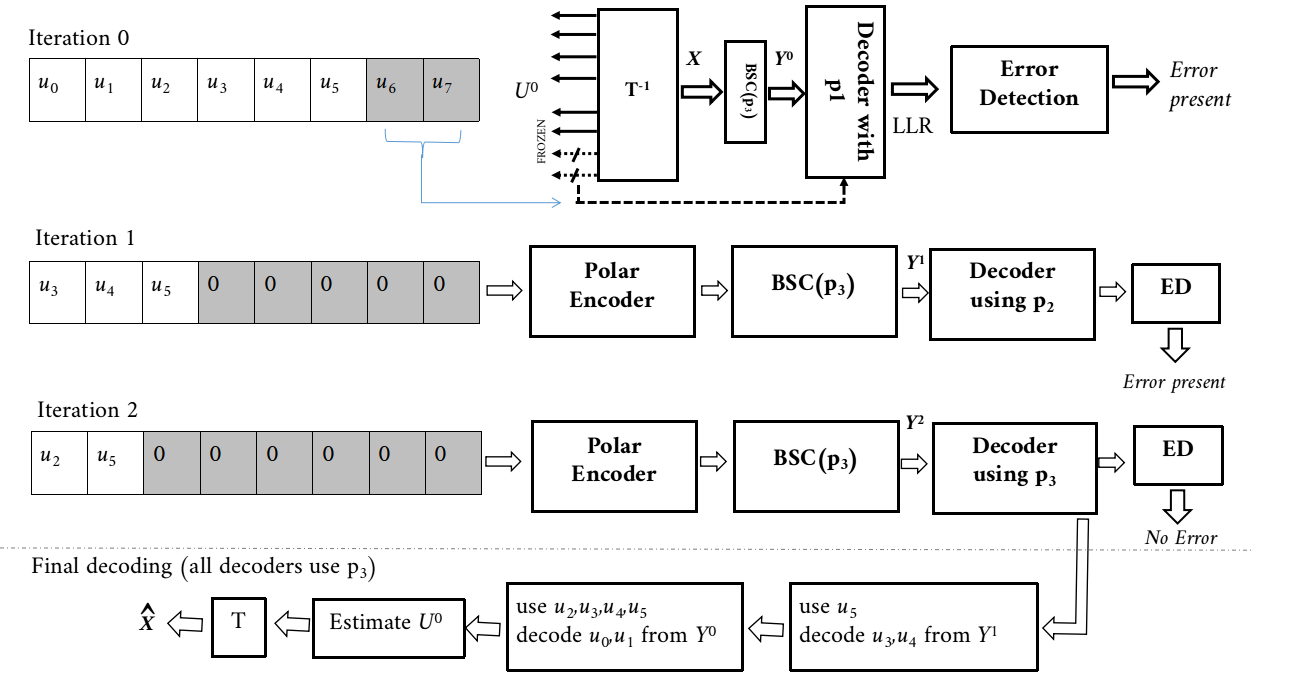
\includegraphics[width=1\textwidth]{iswrpc.png}
  \end{center}
  \caption{Example of Iterative SW compression with Incremental Freezing.}
  \label{fig:iswrpc}
\end{figure} 
Here, a compound BSC channel $\mathcal{C}=\{ p_1 \leq p_2 \leq p_3 \leq p_4\}$ is considered, where $p_i$ is the flipover probability of channel $i$. It is assumed that the rates supported by the channels are $\{ R_1=R, R_2= R/2,R_3= R/3,R_4= R/4\}$. The actual channel in the example is BSC($p_3$), henceforth, we shall denote this as BSC($p_{channel}$). The vector channel is manufactured by polarization of $N$ such BSC($p_{channel}$) channels.
\paragraph{First Iteration:} In the first iteration, the SW compression with Polar Coding scheme suggested in figure \ref{fig:pswscheme} is followed. Additionally, the soft outputs (LLRs) generated from the decoder block are passed through an error-detection (ED) block. In case error is present, receiver replies with a NACK and further iterations are commenced. The decoder \emph{guesses} the channel to be BSC($p_1$) greedily and computes LLR accordingly. Henceforth, we shall denote this as BSC($p_{guess}$). Note, in this case the frozen bits are non-zero, and are communicated error-free to receiver, unlike in the channel coding scenario in figure \ref{fig:if}.
\paragraph{Subsequent Iterations:}In the subsequent iterations, the decoder makes greedy guesses about the channel from a subset of the compound channel which does not include previous guesses. In other words, in second iteration $p_{guess}=p_2$, in third $p_{guess}=p_3$. Iterations continue as long as the ED does not declare error-free transmission, which is communicated as ACK by the receiver.\\
The error-free transmission in these iterations consist of information bits which are suspected to be sent unreliably in previous iterations under impression that present $p_{guess}$ is correct. 
\paragraph{Final Decoding:}When the ED declares no error the decoder infers that the $p_{channel}=p_{guess}$, let us denote this as $p_{final}$. The decoder now  decodes the received channel output vector using $p_{final}$ and considering the bits transmitted error-free in all the iterations as frozen. Finally, with Arikan transform X is estimated.
Note, X and Y have there usual meanings as in figure \ref{fig:swcomp}. 


\subsection{PHY Layer Error Detection} 

A difference between use of Polar Codes for error control and that for SW compression is that, in the latter case the $U_N$ is generated from $X_N$. Hence using a CRC in $U_N$ which can be exploited for error detection and retransmission in Incremental Freezing does not remain feasible.\\This necessitates an error detection scheme which is free of CRC and works in PHY layer. At a high level the ED scheme can be viewed as a hypothesis testing problem for \emph{each iteration} where,
\begin{align*}
\mathcal{H}_0 & :\text{The channel is the current guess, i.e., } p_{channel}=p_{guess}\\
\mathcal{H}_1 & :\text{The channel is worse, i.e., } p_{channel} > p_{guess}
\end{align*}

It is understood that due to the sequential and greedy nature of Inc-Frz, cases where $p_{channel} < p_{guess}$ need not be considered. Since the magnitude of the LLR dictates the error probability of corresponding bit, a hypothesis test based on $|LLR|$ has been proposed.

\subsubsection{The Error Detection Test }
Consider the setting as in section \ref{adapt}. Let there be $K$ good bit-channels after polarization.  
Since Inc-Frz guesses the best channel first, we can say that at $j^{th}$ iteration $p_{guess}=p_j$. 
Let $\Lambda_j^i(k)$ be the magnitude of the LLR of $k^{th}$ bit-channel, $k\in{1,2,...N}$ at the output of the decoder at the end of $j^{th}$ iteration such that $p_{guess}=p_j$ for $p_{channel}=p_i$. Empirical distribution of $\Lambda_j^i(k)$ based on a simulation has been shown in figure \ref{fig:absllr}.
\begin{figure}[h]
 \begin{center}
    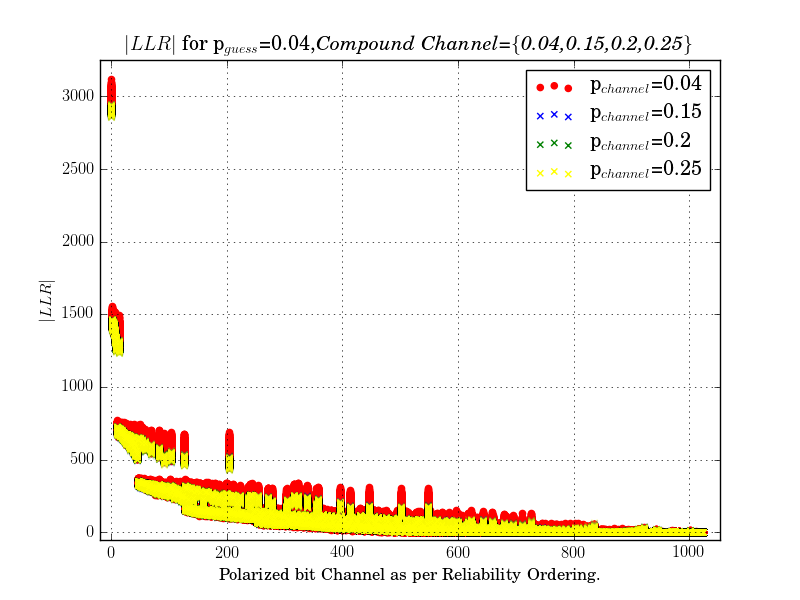
\includegraphics[width=1\textwidth]{absllr0p04.png}
  \end{center}
  \caption{$|LLR|$ for $p_{guess}=0.04$ and $p_{channel} \in \mathcal{C}$.}
  \label{fig:absllr}
\end{figure}\\
Thus, the hypotheses may be restated as,
\begin{align*}
\mathcal{H}_0 & :j=i\\
\mathcal{H}_1 & :j<i
\end{align*}
Note that, for $j < i$, $p_i > p_j$. Hence, the true channel is worse and further iterations are needed. Two tests have been suggested based on statistics which are functions of  $\Lambda_j^i(k)$ in the following subsection.

\subsubsection{Proposed Tests}
\paragraph{TEST 1: All good channels are above a given threshold.} Initially, a test was considered where $p_{guess}=p_{channel}$ is declared if the |LLR| of all the good channels clear a given threshold under the current guess. That is, after $j^{th}$ iteration,
\begin{align*}  
j & =i, 
\begin{cases}
\text{   if, }  \Lambda_{j}^i(k) > \lambda, \forall k \in {1,2,3...K}\\
\text{alternatively, } \displaystyle\min_{k \in [K]}\Lambda_{j}^i(k) > \lambda  \\
\end{cases}\\
 j & < i,  \text{ o.w.}
\end{align*} 
Here $\lambda$ is chosen to reflect the required reliability. As it can be seen in figure \ref{fig:absllr}, the support of the distributions of $\Lambda_{j=i}^i(k)$ and $\Lambda_{j \neq i}^i(k)$ overlap considerably and $\Lambda_{j=i}^i(k)$ has a higher variance. This gave rise to high missed detection probability $P_M$, which resulted in premature termination of the Inc-Frz scheme and high probability of error. Here, $P_M=P_1(p_i>p_j)$ indicates the probability that the test declares a better channel as the true channel.
\newpage
\paragraph{TEST 2: A given fraction of good channels are above a threshold.}  
In this test $p_{guess}=p_{channel}$ is declared if the |LLR| of a certain fraction of the good channels clear a threshold. The fraction is dependent on the iteration number. After $j^{th}$ iteration,
\begin{align*}  
j &=i,
 \text{   if, } \frac{1}{K}\sum^K_{k=1} \mathbbm{1}_{\{\Lambda_{j}^i(k) > \lambda\}} > \Theta_j \\
j & < i,  \text{ o.w. }
\end{align*} 
The results of Monte-Carlo simulation for estimating $P_M$ and $P_F$ for $\mathcal{C}=\{p_1=0.04,p_2=0.15,p_3=0.2,p_4=0.25\}$ is shown in figure \ref{fig:theta1},\ref{fig:theta2}, \ref{fig:theta3}. Note, in the figures $\Theta$ is considered to be percentage.
\begin{figure}[h]
 \begin{center}
    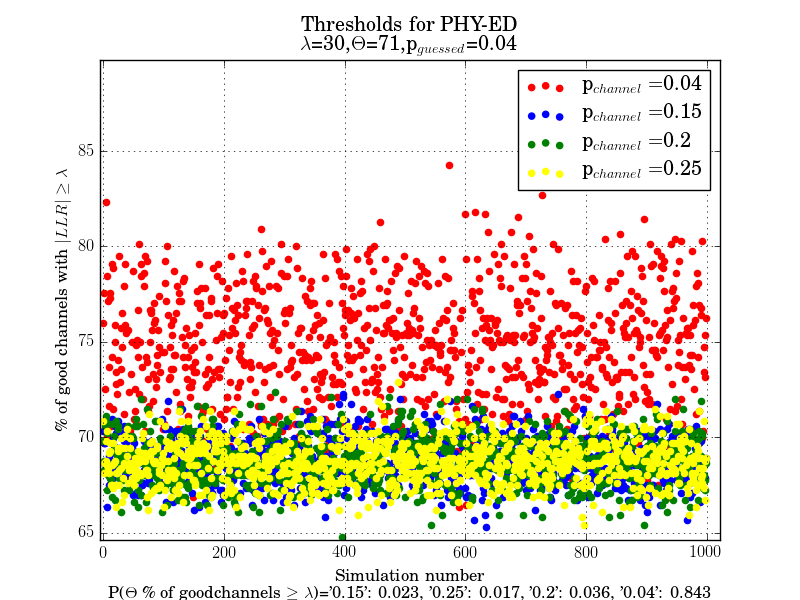
\includegraphics[width=1\textwidth]{theta0p04.png}
  \end{center}
  \caption{$P_M$ and $P_F$ estimation for ED after $1^{st}$ iteration, $p_{guess}=0.04$.}
  \label{fig:theta1}
\end{figure}\\
From figure \ref{fig:theta1}, the detection error probabilities for the first  iteration can be calculated as $P_F=0.16$ and $P_M=0.06$. For the values of $\Theta$ used, $P_F\approx0.4$  for second and third iteration with $P_M\approx0.13$. A higher value of $P_F$ does not affect the frame error probabilities but causes rate loss. Though higher value of $P_M$ affects frame error probabilities adversely, it should be noted that the detection error probabilities in later iterations are weighted by that of the previous ones and hence this effect diminishes with iteration.
\begin{figure}[h]
\centering
\begin{subfigure}{0.5\textwidth}
    \centering
    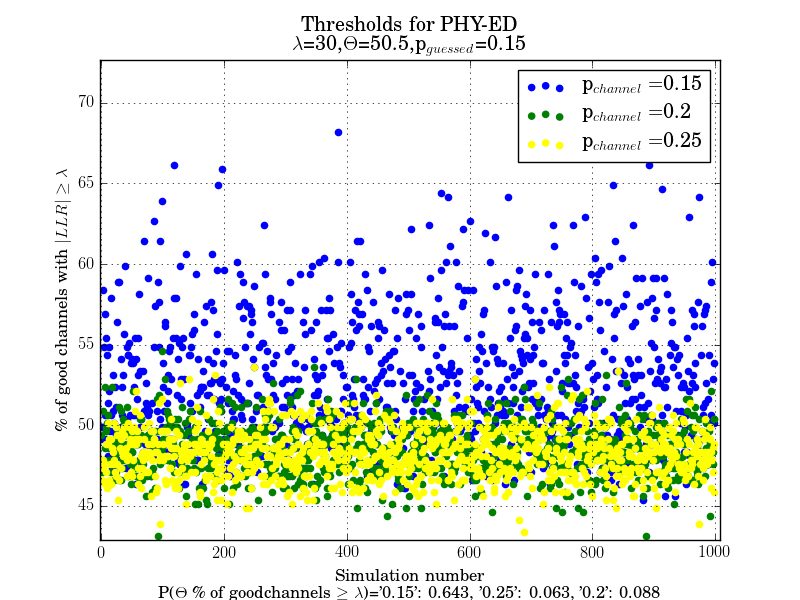
\includegraphics[width=1.1\textwidth]{theta0p15new.png}
    \caption{ED after $2^{nd}$ iteration.}
    \label{fig:theta2}
\end{subfigure}
\begin{subfigure}{0.5\textwidth}
    \centering
    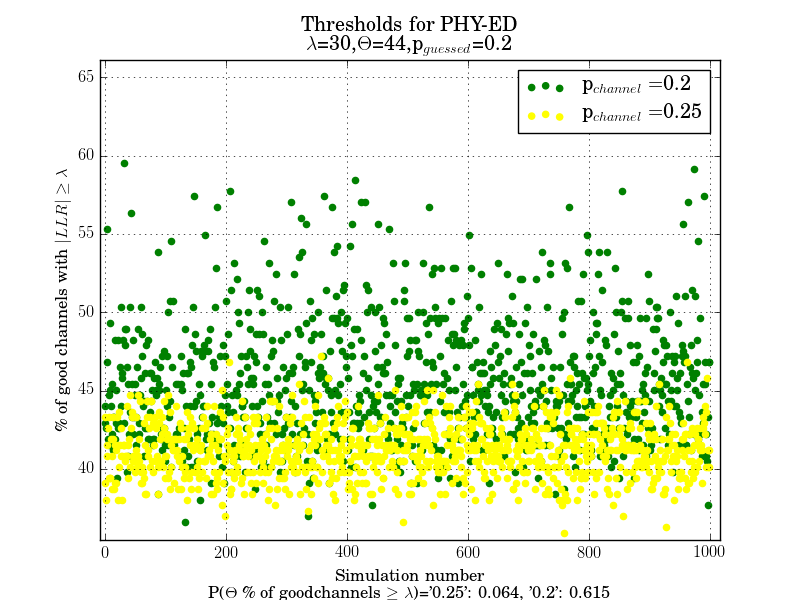
\includegraphics[width=1.1\textwidth]{theta0p2.png}
    \caption{ED after $3^{rd}$ iteration.}
    \label{fig:theta3}
\end{subfigure}
\caption{$P_M$ and $P_F$ estimation for ED after $2^{nd}$ and $3^{rd}$ iteration.}
\label{fig:theta23}
\end{figure}

\clearpage
\subsection{Performance Evaluation}
%-------------------------------SW
Simulation results for the scheme in figure \ref{fig:iswrpc} used for iterative SW compression with Inc-Frz and PHY-ED are presented in figure \ref{fig:fersw1}, \ref{fig:fersw2}, \ref{fig:fersw3} and \ref{fig:fersw4}.
Each plot corresponds to a fixed channel with $p_{channel} \in \mathcal{C}$. The performance of Polar Codes designed for the specific $p_{channel}$ has been given for comparison. Figure \ref{fig:perfch} shows similar results for Rateless Polar Coding with Inc-Frz and PHY-ED.\\
Let $K$ be the number of bit-channels assumed to be good at the first iteration. For simulation, $K$ is varied from $0$ to $K^*$ such that $K^*/N$ is the capacity of the best channel.\\ In case of Rateless Polar Coding, the scheme uses iterations to communicate these $K$ bits, thus achieving some rate and corresponding frame error rate (FER). In case of SW compression the number of bits that remain unfrozen after the final iteration divided by $N$ is viewed as the achieved rate. The FER has been plotted against the achieved rates for performance evaluation. The plots capture the error detection and retransmission action which results in change in effective block length of the code. Figure \ref{fig:rlsw} captures the rate loss seen for varying $p_{channel}$.  
\begin{figure}[h!]
 \begin{center}
    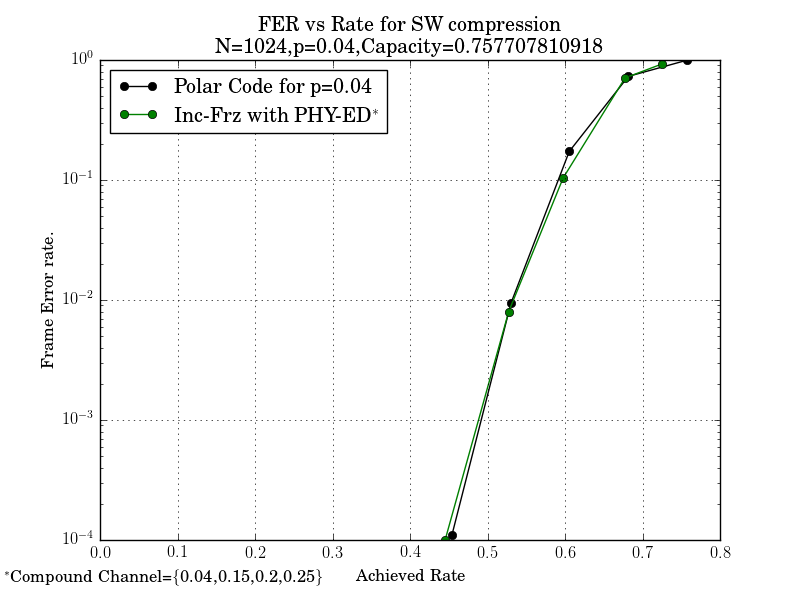
\includegraphics[width=0.7\textwidth]{FERSW_0p04.png}
  \end{center}
  \caption{FER vs Rate for SW compression with $p_{channel}=0.04$}
  \label{fig:fersw1}
\end{figure}
\begin{figure}[h!]
 \begin{center}
    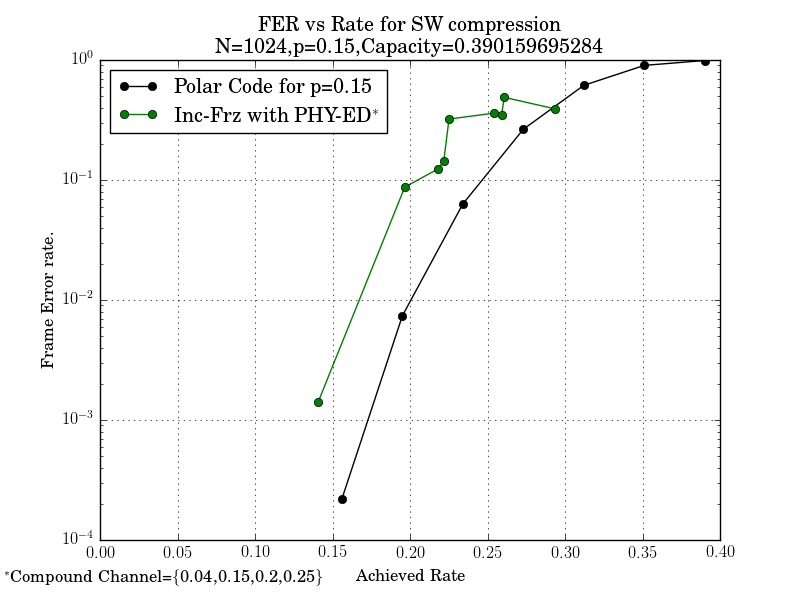
\includegraphics[width=0.7\textwidth]{FERSW_0p15.png}
  \end{center}
  \caption{FER vs Rate for SW compression with $p_{channel}=0.15$ }
  \label{fig:fersw2}
\end{figure}
\begin{figure}[h!]
 \begin{center}
    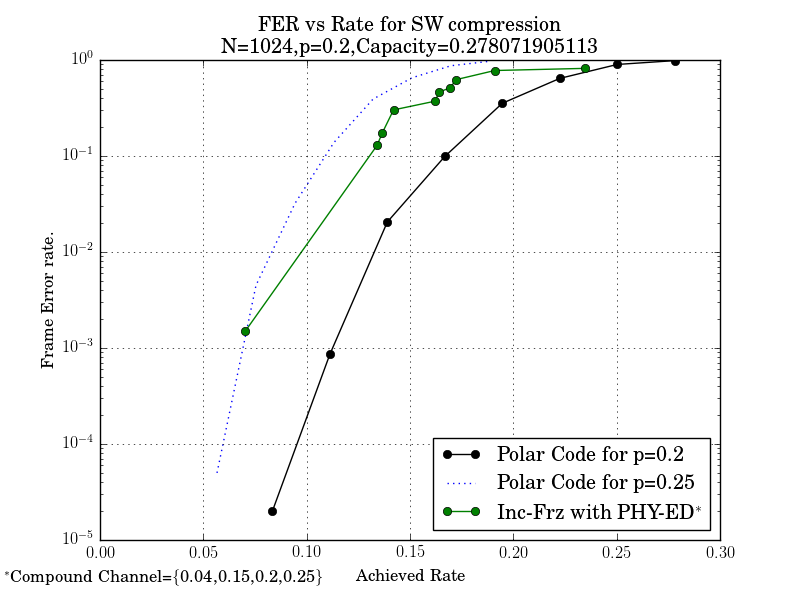
\includegraphics[width=0.7\textwidth]{FERSW_0p2.png}
  \end{center}
  \caption{FER vs Rate for SW compression with $p_{channel}=0.2$ }
  \label{fig:fersw3}
\end{figure}
\begin{figure}[h!]
 \begin{center}
    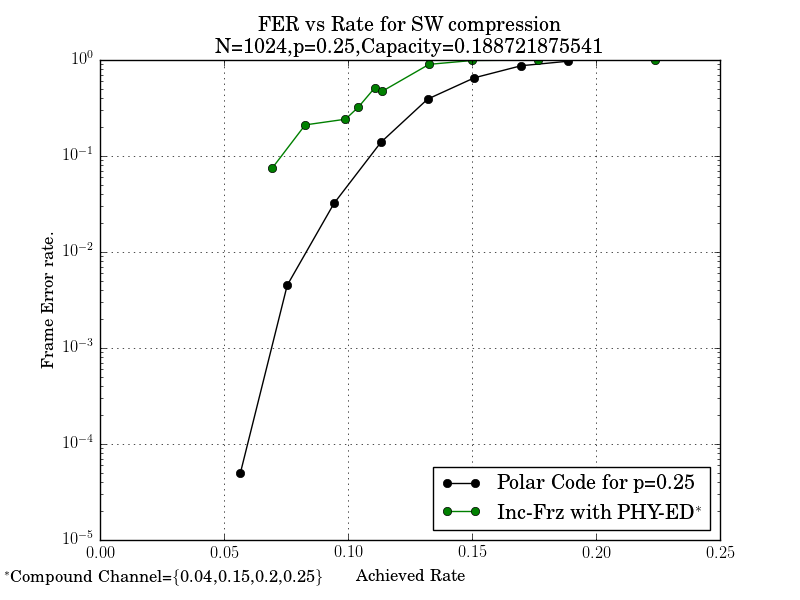
\includegraphics[width=0.7\textwidth]{FERSW_0p25.png}
  \end{center}
  \caption{FER vs Rate for SW compression with $p_{channel}=0.25$ }
  \label{fig:fersw4}
\end{figure}
\begin{figure}[h!]
 \begin{center}
    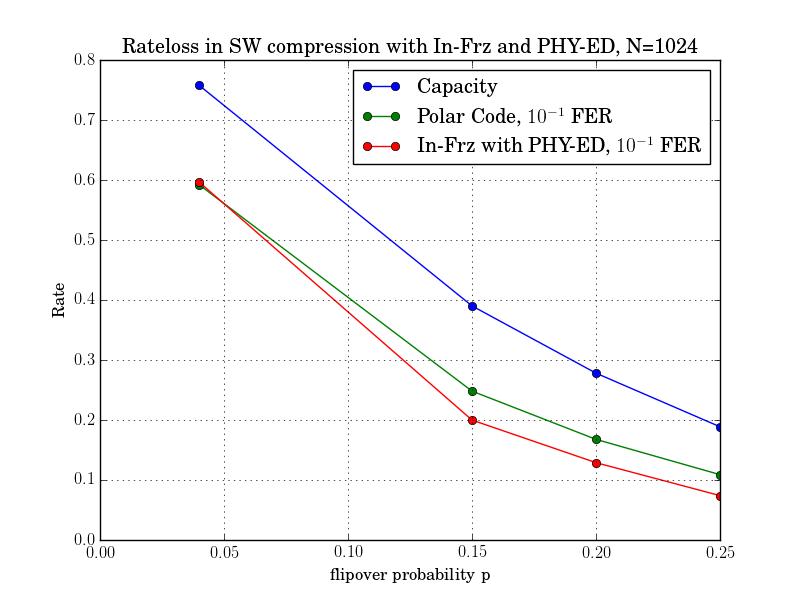
\includegraphics[width=0.7\linewidth]{ratelosssw.png}
  \end{center}
  \caption{Rate loss for SW compression with Inc-Frz.}
  \label{fig:rlsw}
\end{figure}
%----------------------------------channel
\clearpage
\begin{figure}[h]
\centering
\begin{subfigure}{.5\textwidth}
  \centering
  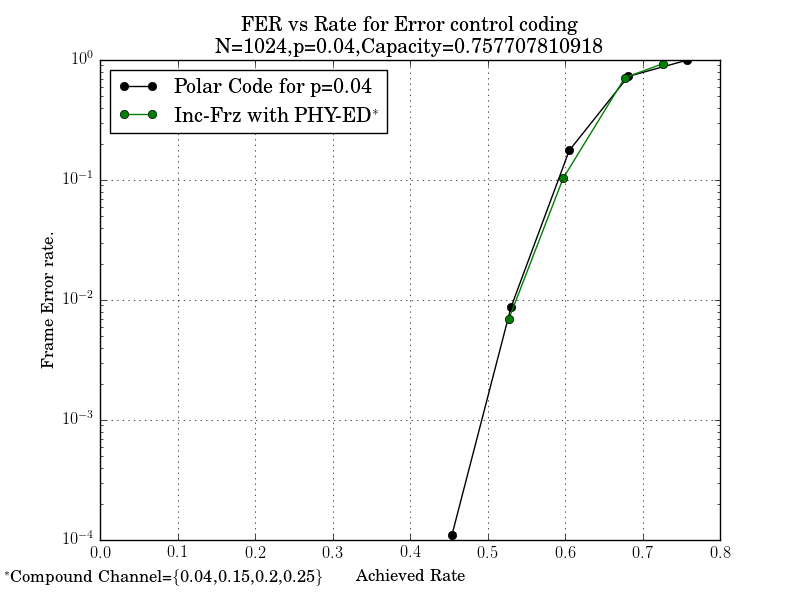
\includegraphics[width=1.1\linewidth]{FER_channel0p04.png}
  \caption{FER vs Rate for $p_{channel}=0.04$}
  \label{fig:pch1}
\end{subfigure}%
\begin{subfigure}{.5\textwidth}
  \centering
  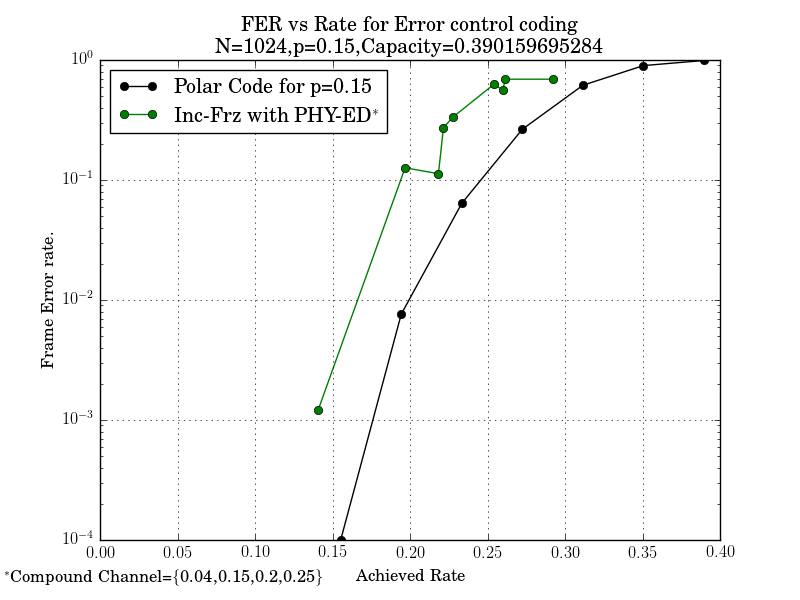
\includegraphics[width=1.1\linewidth]{FER_channel0p15.png}
  \caption{FER vs Rate for $p_{channel}=0.15$}
  \label{fig:pch2}
\end{subfigure}
\begin{subfigure}{.5\textwidth}
  \centering
  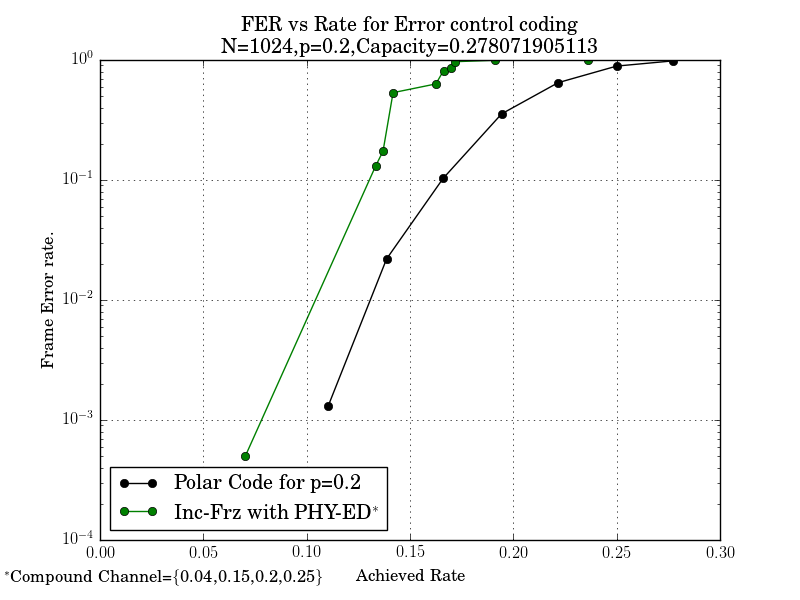
\includegraphics[width=1.1\linewidth]{FER_channel0p2.png}
  \caption{FER vs Rate for $p_{channel}=0.2$}
  \label{fig:pch3}
\end{subfigure}%
\begin{subfigure}{.5\textwidth}
  \centering
  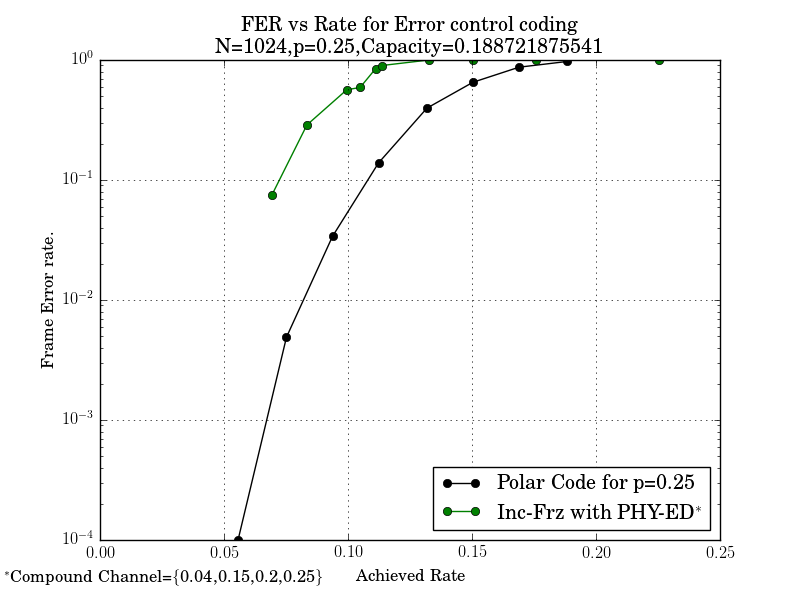
\includegraphics[width=1.1\linewidth]{FER_channel0p25.png}
  \caption{FER vs Rate for $p_{channel}=0.25$}
  \label{fig:pch4}
\end{subfigure}
\begin{subfigure}{.5\textwidth}
  \centering
  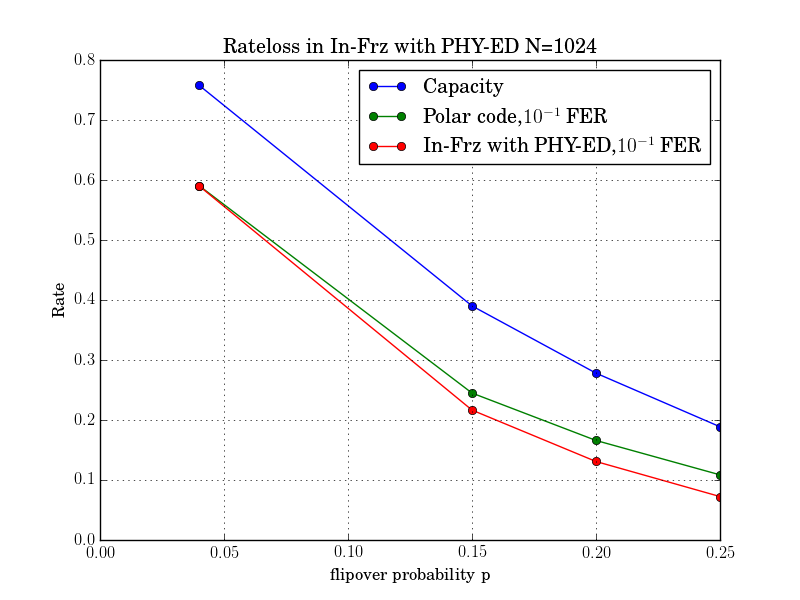
\includegraphics[width=1.1\linewidth]{rateloss_channel.png}
  \caption{Rate loss in Inc-Frz with PHY-ED}
  \label{fig:rlch}
\end{subfigure}
\caption{Performance Evaluation of Rateless Polar Coding with Inc-Frz and PHY-ED.}
\label{fig:perfch}
\end{figure}
%--------------------------------------------------------------------------
% CONCLUSION AND FUTURE WORK
%--------------------------------------------------------------------------
\clearpage
\section{Conclusion and Future work}\label{future}
\begin{itemize}
\item The proposed scheme is an implementable solution to the \emph{Data-Exchange} problem.
\item It reduces the communication among nodes.
\item The CRC-free universal polar code promises considerable rate gain for communication using short packet lengths. 
\item There are few channels which are good for use during the entire transmission. Communicating critical data over these channel ensure high reliability and availability . 
\end{itemize}
\begin{itemize}
\item Future work.
\begin{itemize}
\item Extensive performance analysis and theoretical analysis of proposed error detection scheme as a RB-HARQ for Polar Codes.
\item Implementation of the scheme for multiparty data exchange.
\end{itemize}
\end{itemize}




%----------------------------------------------------------------------------------------
%	BIBLIOGRAPHY
%----------------------------------------------------------------------------------------
\clearpage
%\renewcommand{\refname}{\spacedlowsmallcaps{References}} % For modifying the bibliography heading

\bibliographystyle{unsrt}

\bibliography{polarmid.bib} % The file containing the bibliography

%----------------------------------------------------------------------------------------

\end{document}